\chapter{立体化学：手性与异构}\label{ch:g12:stereochemistry}

留兰香叶与葛缕子籽闻起来毫不相似：一种是口香糖般的清新气味，
另一种是黑麦面包般的醇香。然而，
产生这两种气味的\omterm{def:g7:atoms-and-molecules:molecule}{分子}是同一种香芹酮，
由相同的\omterm{def:g7:atoms-and-molecules:atom}{原子}按相同的顺序成键构成。两种香芹酮的差别，只在于如同左手与右手之别：
二者互为镜像。
我们的鼻子由本身“有\omterm{def:g12:stereochemistry:chiral}{手性}”的\omterm{def:g7:atoms-and-molecules:molecule}{分子}构成，能够将二者区分开。
本章学习从三维空间的角度看待\omterm{def:g7:atoms-and-molecules:molecule}{分子}。

\begin{recall}
\omterm{def:g7:atoms-and-molecules:molecule}{分子}的形状，以及用楔形线和虚线在空间中画出\omterm{def:g7:atoms-and-molecules:molecule}{分子}的方式
（见\cref{ch:g10:lewis-and-shape}）。\omterm{def:g11:organic-skeletons:isomer}{构造异构体}
（见\cref{ch:g11:organic-skeletons}）。\omterm{def:g11:functional-groups:functional-group}{官能团}
（见\cref{ch:g11:functional-groups}）。
\end{recall}

\begin{omfigure}
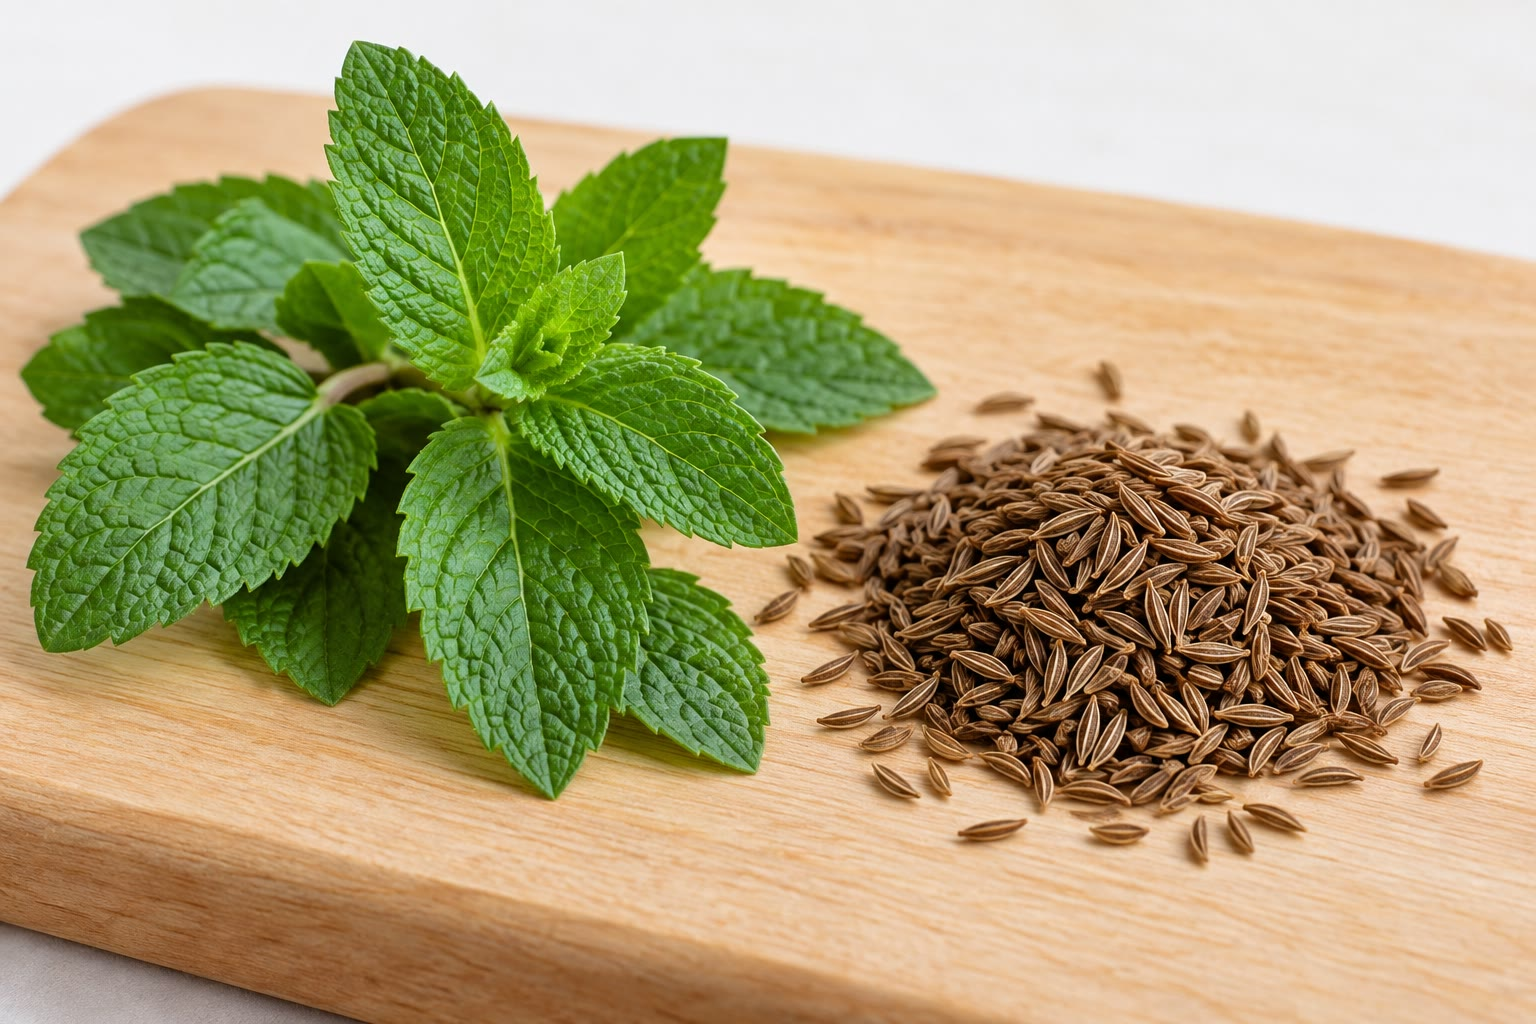
\includegraphics[width=0.48\linewidth]{images/book1/ai/g12-mint-caraway.jpg}

{\small 留兰香与葛缕子：两个互为镜像的\omterm{def:g7:atoms-and-molecules:molecule}{分子}，两种气味。}
\end{omfigure}

\section{空间中的分子}

\begin{definition}[立体异构体]\label{def:g12:stereochemistry:stereoisomer}
\emph{立体异构体}\index{立体异构体}是指具有相同
\omterm{def:g11:organic-skeletons:formulas}{分子式}、相同成键\omterm{def:g7:atoms-and-molecules:atom}{原子}顺序的\omterm{def:g7:atoms-and-molecules:molecule}{分子}，它们仅在
\omterm{def:g7:atoms-and-molecules:atom}{原子}的空间排列上不同。
\end{definition}

\begin{definition}[楔形式]\label{def:g12:stereochemistry:cram}
在\emph{楔形式}\index{楔形式}中，表示带有四个单键的碳\omterm{def:g7:atoms-and-molecules:atom}{原子}时，
其中两个键以普通线段画在纸面上，相互成一定夹角；
指向读者的键画成实楔形，
背离读者的键画成虚楔形。
\end{definition}

\section{手性}

\begin{definition}[手性、手性碳原子]\label{def:g12:stereochemistry:chiral}
若一个物体或\omterm{def:g7:atoms-and-molecules:molecule}{分子}不能与其镜像重合，如同人的左右手，则称其具有
\emph{手性}\index{手性}。与四个互不相同的\omterm{def:g7:atoms-and-molecules:atom}{原子}或基团相连的碳\omterm{def:g7:atoms-and-molecules:atom}{原子}
称为\emph{手性碳原子}\index{手性碳原子}
，常用星号标记。
\end{definition}

\begin{proposition}[一个手性碳原子使分子具有手性]\label{prop:g12:stereochemistry:one-carbon}
含有且仅含一个\omterm{def:g12:stereochemistry:chiral}{手性碳原子}的\omterm{def:g7:atoms-and-molecules:molecule}{分子}具有\omterm{def:g12:stereochemistry:chiral}{手性}。
\end{proposition}

\begin{proof}
在本阶段不加证明地承认：交换围绕\omterm{def:g12:stereochemistry:chiral}{手性碳原子}的四个不同基团中的两个，
便得到其镜像，且整个\omterm{def:g7:atoms-and-molecules:molecule}{分子}无论怎样旋转，
都无法使镜像与原\omterm{def:g7:atoms-and-molecules:molecule}{分子}重合，因为四个基团全不相同。
\end{proof}

\begin{definition}[对映异构体、外消旋混合物]\label{def:g12:stereochemistry:enantiomer}
两种互为镜像且不能重合的\omterm{def:g12:stereochemistry:stereoisomer}{立体异构体}，
互为\emph{对映异构体}\index{对映异构体}。等量的
两种对映异构体的\omterm{def:g6:pure-substances-and-mixtures:mixture}{混合物}，称为\emph{外消旋
混合物}\index{外消旋混合物}。
\end{definition}

\begin{omfigure}
\setchemfig{atom sep=2.2em}
\begin{tikzpicture}[font=\small]
  \node at (-2.4,0) {\chemfig{C(-[2]COOH)(-[4]H_3C)(<[:-30]OH)(<:[:-150]H)}};
  \node at (2.4,0) {\chemfig{C(-[2]COOH)(-[0]CH_3)(<[:-150]HO)(<:[:-30]H)}};
  \draw[dashed, omDef, thick] (0,-1.5) -- (0,1.6) node[above] {镜面};
  \node[anchor=north] at (-2.4,-1.4) {乳酸，A};
  \node[anchor=north] at (2.4,-1.4) {其镜像，B};
\end{tikzpicture}

{\small 乳酸（\ce{CH3-CH(OH)-COOH}）的两种\omterm{def:g12:stereochemistry:enantiomer}{对映异构体}，以
\omterm{def:g12:stereochemistry:cram}{楔形式}表示。中心碳\omterm{def:g7:atoms-and-molecules:atom}{原子}为\omterm{def:g12:stereochemistry:chiral}{手性碳原子}（\ce{H}、\ce{OH}、
\ce{CH3}、\ce{COOH}）。任何旋转都无法使 A 变为 B，二者
的差别如同左手与右手。}
\end{omfigure}

\begin{method}[分子是否具有手性？]\label{met:g12:stereochemistry:chiral}
\begin{enumerate}
  \item 寻找\omterm{def:g12:stereochemistry:chiral}{手性碳原子}：即连有四个不同
        基团的碳\omterm{def:g7:atoms-and-molecules:atom}{原子}。若没有，则该\omterm{def:g7:atoms-and-molecules:molecule}{分子}（在本书中）不具有\omterm{def:g12:stereochemistry:chiral}{手性}。
  \item 恰有一个：该\omterm{def:g7:atoms-and-molecules:molecule}{分子}具有\omterm{def:g12:stereochemistry:chiral}{手性}。
  \item 两个或更多：寻找一个能将\omterm{def:g7:atoms-and-molecules:molecule}{分子}分为两个
        互为镜像的两半的平面，可以是其某一\omterm{def:g12:stereochemistry:conformation}{构象}中的平面；若存在，
        则该\omterm{def:g7:atoms-and-molecules:molecule}{分子}不具有\omterm{def:g12:stereochemistry:chiral}{手性}，否则具有\omterm{def:g12:stereochemistry:chiral}{手性}。
\end{enumerate}
\end{method}

\begin{remark}[性质相同，气味不同]\label{rem:g12:stereochemistry:same}
% ledger: smell:carvone-R, smell:carvone-S
两种\omterm{def:g12:stereochemistry:enantiomer}{对映异构体}具有相同的熔点与沸点、相同的
\omterm{def:g6:solutions-and-solubility:solubility}{溶解度}与光谱：任何以非\omterm{def:g12:stereochemistry:chiral}{手性}物质进行的测量，
对二者都给出相同的结果。二者的差别仅在于
与\omterm{def:g12:stereochemistry:chiral}{手性}物质相遇时才会显现，例如偏振光，二者能使其
偏振面向相反方向旋转，或与鼻中的受体相互作用：一种香芹酮
闻起来带有留兰香味，其\omterm{def:g12:stereochemistry:enantiomer}{对映异构体}则带有葛缕子的气味。
\end{remark}

\section{非对映异构体}

\begin{definition}[非对映异构体]\label{def:g12:stereochemistry:diastereomer}
彼此不互为镜像的\omterm{def:g12:stereochemistry:stereoisomer}{立体异构体}，称为
\emph{非对映异构体}\index{非对映异构体}。与\omterm{def:g12:stereochemistry:enantiomer}{对映异构体}不同，
其物理性质各不相同。
\end{definition}

\begin{proposition}[立体异构体的计数]\label{prop:g12:stereochemistry:count}
含有 $n$ 个\omterm{def:g12:stereochemistry:chiral}{手性碳原子}的\omterm{def:g7:atoms-and-molecules:molecule}{分子}，至多有 $2^n$ 种\omterm{def:g12:stereochemistry:stereoisomer}{立体异构体}。
若\omterm{def:g7:atoms-and-molecules:molecule}{分子}具有两个相同的部分，则\omterm{def:g12:stereochemistry:stereoisomer}{立体异构体}的数目更少：此时其中一种
组合具有镜面而不具\omterm{def:g12:stereochemistry:chiral}{手性}（为\emph{内消旋}形式）。
\end{proposition}

\begin{proof}
每个\omterm{def:g12:stereochemistry:chiral}{手性碳原子}可有两种排列，且彼此独立，
共有 $2 \times 2 \times \dots \times 2 = 2^n$ 种组合。当两种
组合为同一\omterm{def:g7:atoms-and-molecules:molecule}{分子}时，数目减少。
\end{proof}

\begin{omfigure}
\setchemfig{atom sep=1.9em}
\begin{tabular}{ccc}
\chemfig{HOOC-[:-30]C(<[:-90]OH)-[:30]C(<[:90]OH)-[:-30]COOH} &
\chemfig{HOOC-[:-30]C(<:[:-90]OH)-[:30]C(<:[:90]OH)-[:-30]COOH} &
\chemfig{HOOC-[:-30]C(<[:-90]OH)-[:30]C(<:[:90]OH)-[:-30]COOH} \\[4pt]
\small L-酒石酸 & \small D-酒石酸 & \small 内消旋酒石酸 \\
\small （\omterm{def:g12:stereochemistry:chiral}{手性}） & \small （\omterm{def:g12:stereochemistry:chiral}{手性}，为 L 的镜像） & \small （不具\omterm{def:g12:stereochemistry:chiral}{手性}）
\end{tabular}

{\small 酒石酸的三种\omterm{def:g12:stereochemistry:stereoisomer}{立体异构体}。L 与 D 互为
\omterm{def:g12:stereochemistry:enantiomer}{对映异构体}；二者各自都是内消旋形式的\omterm{def:g12:stereochemistry:diastereomer}{非对映异构体}，内消旋形式的一种构型具有镜面：
共三种\omterm{def:g12:stereochemistry:stereoisomer}{立体异构体}，而非 $2^2 = 4$ 种。}
\end{omfigure}

\begin{history}[1848 年巴斯德手工分拣晶体]
1848 年，年轻的化学家路易·巴斯德用放大镜观察
一种“外消旋酸”的盐的晶体，外消旋酸是酒石酸的一种形式，它
不使偏振光向任何方向偏转。他注意到，晶体呈
两种形状，彼此互为镜像，他用
镊子逐粒分拣。\omterm{def:g2:mixing-and-dissolving:dissolve}{溶解}后，一堆使偏振光向右偏转，
另一堆以相同的幅度向左偏转。由此可知，外消旋酸是两种互为镜像的\omterm{def:g7:atoms-and-molecules:molecule}{分子}的\omterm{def:g6:pure-substances-and-mixtures:mixture}{混合物}。
他由此断定，\omterm{def:g7:atoms-and-molecules:molecule}{分子}是有\omterm{def:g12:stereochemistry:chiral}{手性}的。
\end{history}

\begin{omfigure}
\begin{minipage}[t]{0.36\linewidth}\centering
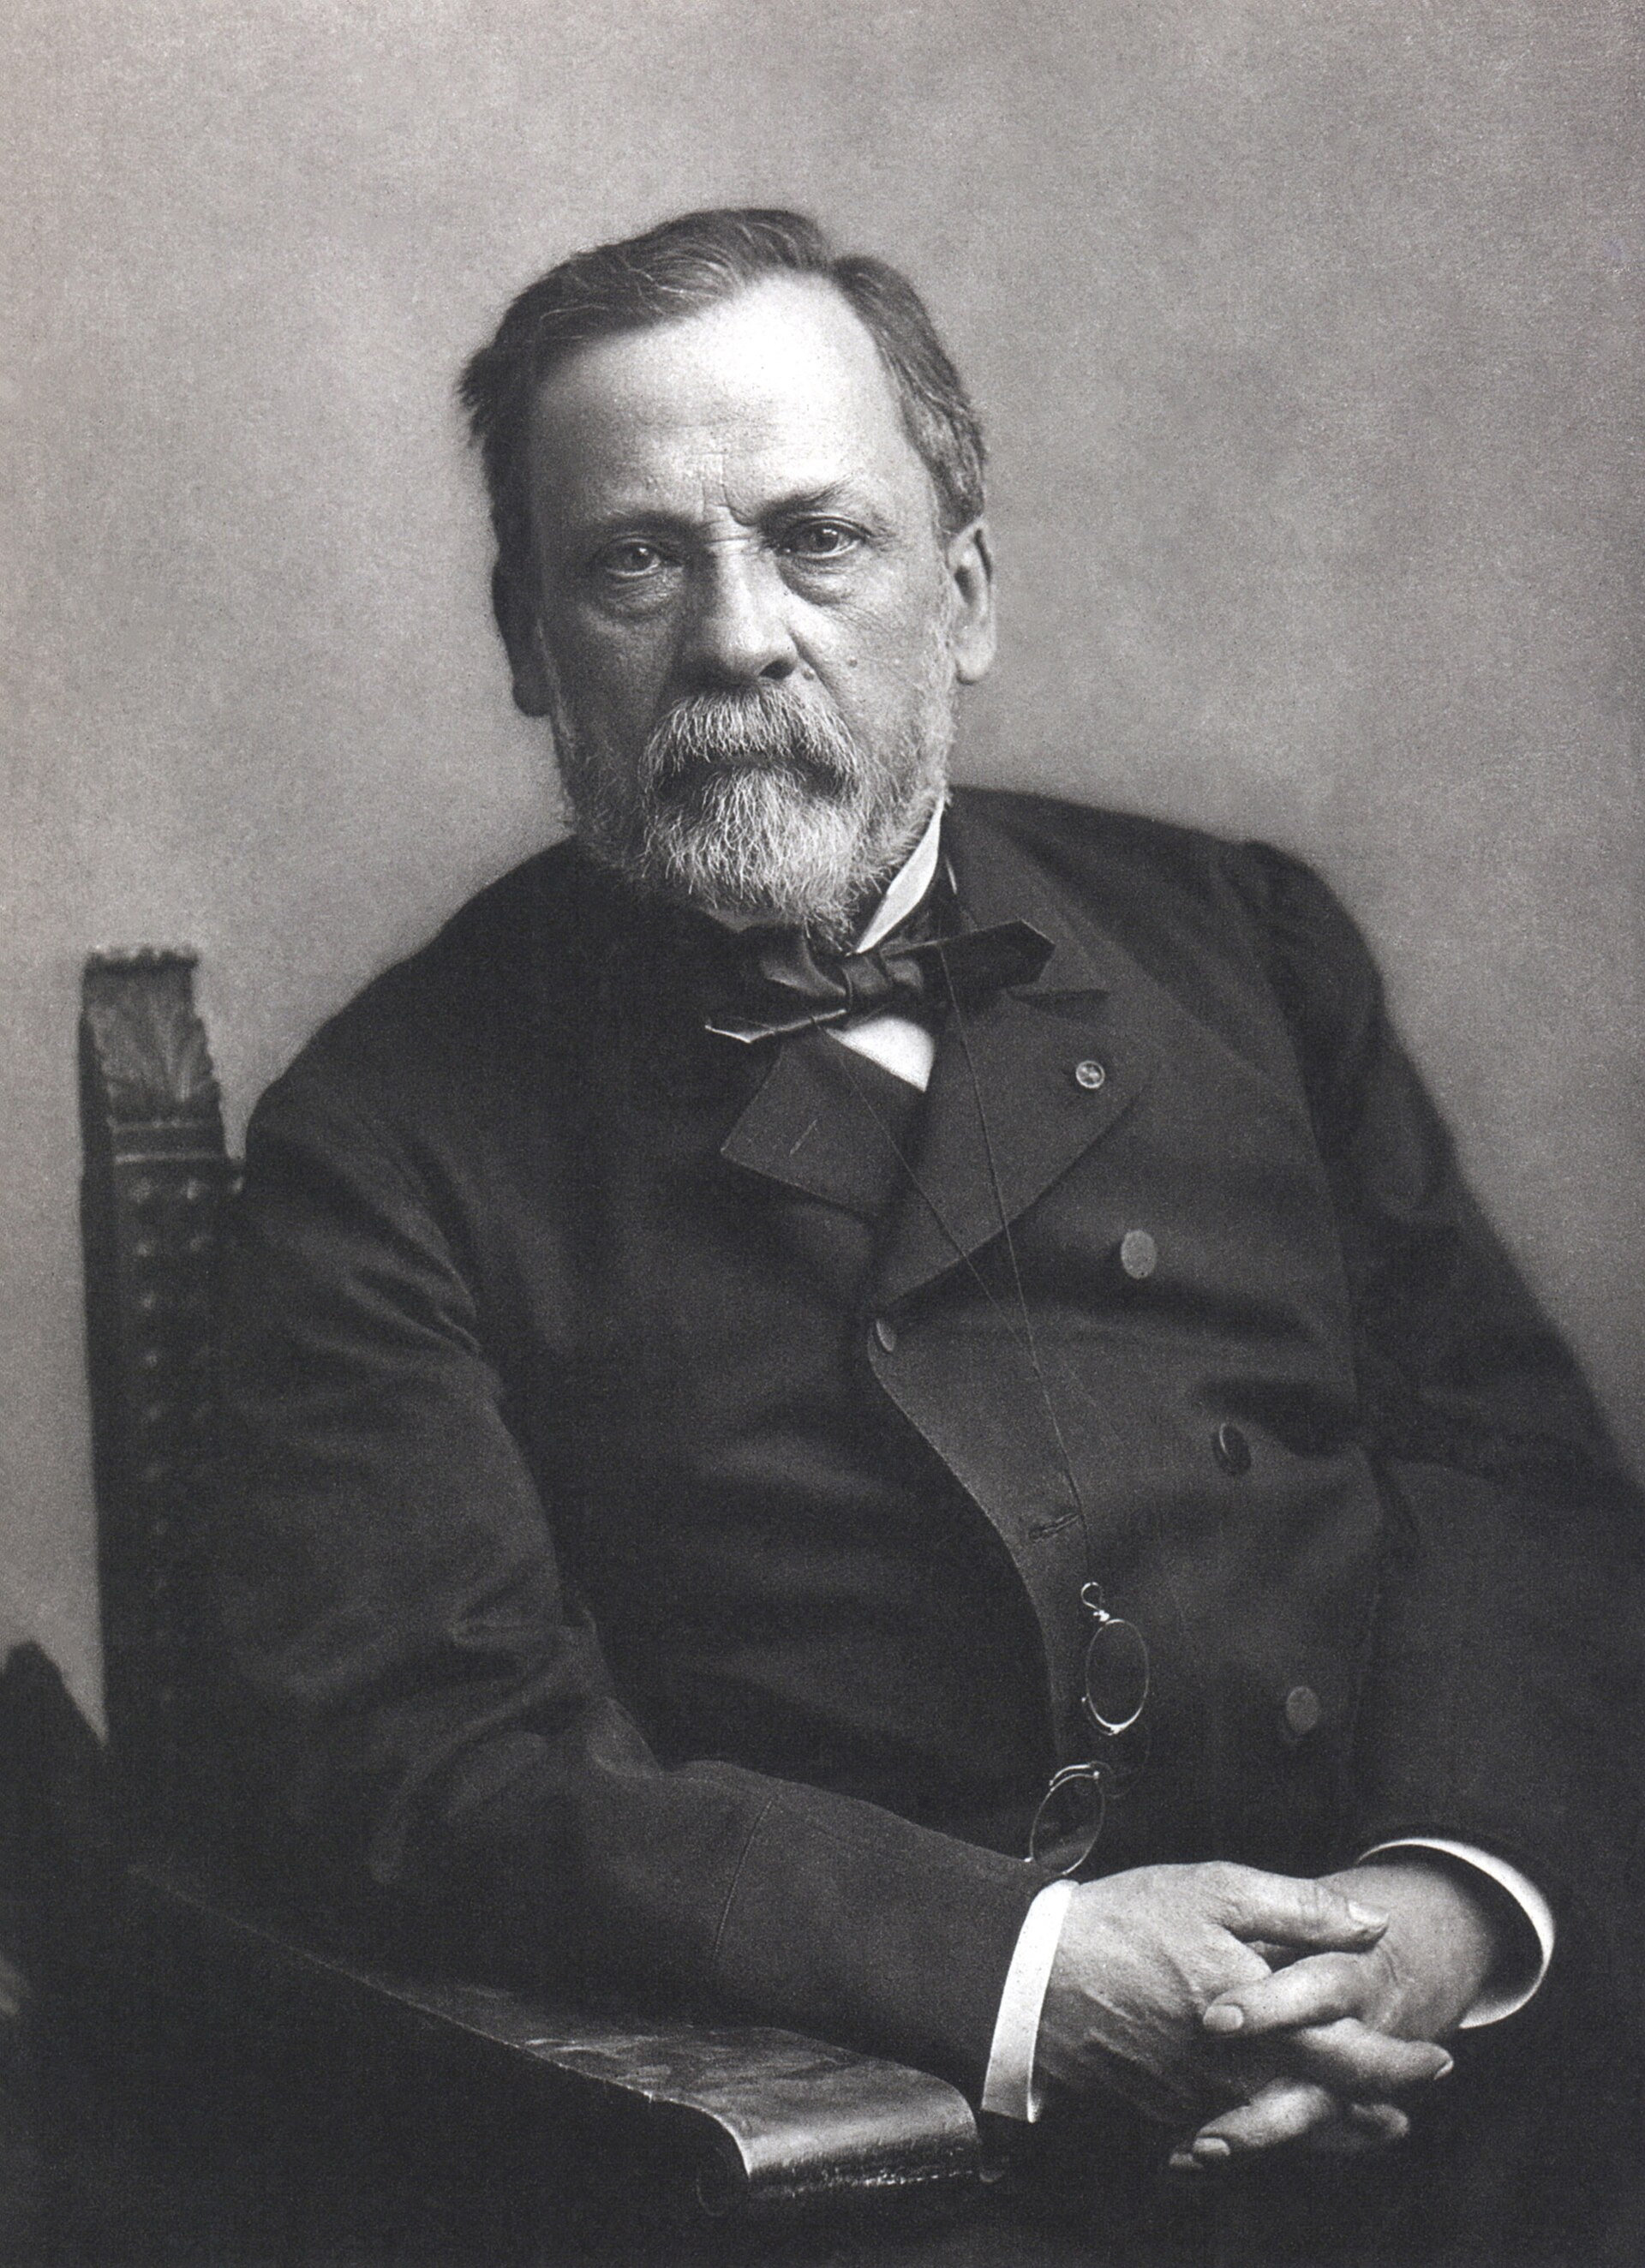
\includegraphics[height=5cm]{images/book1/pasteur.jpg}

{\small 路易·巴斯德（1822--1895）。照片：Paul Nadar。}
\end{minipage}\qquad
\begin{minipage}[t]{0.36\linewidth}\centering
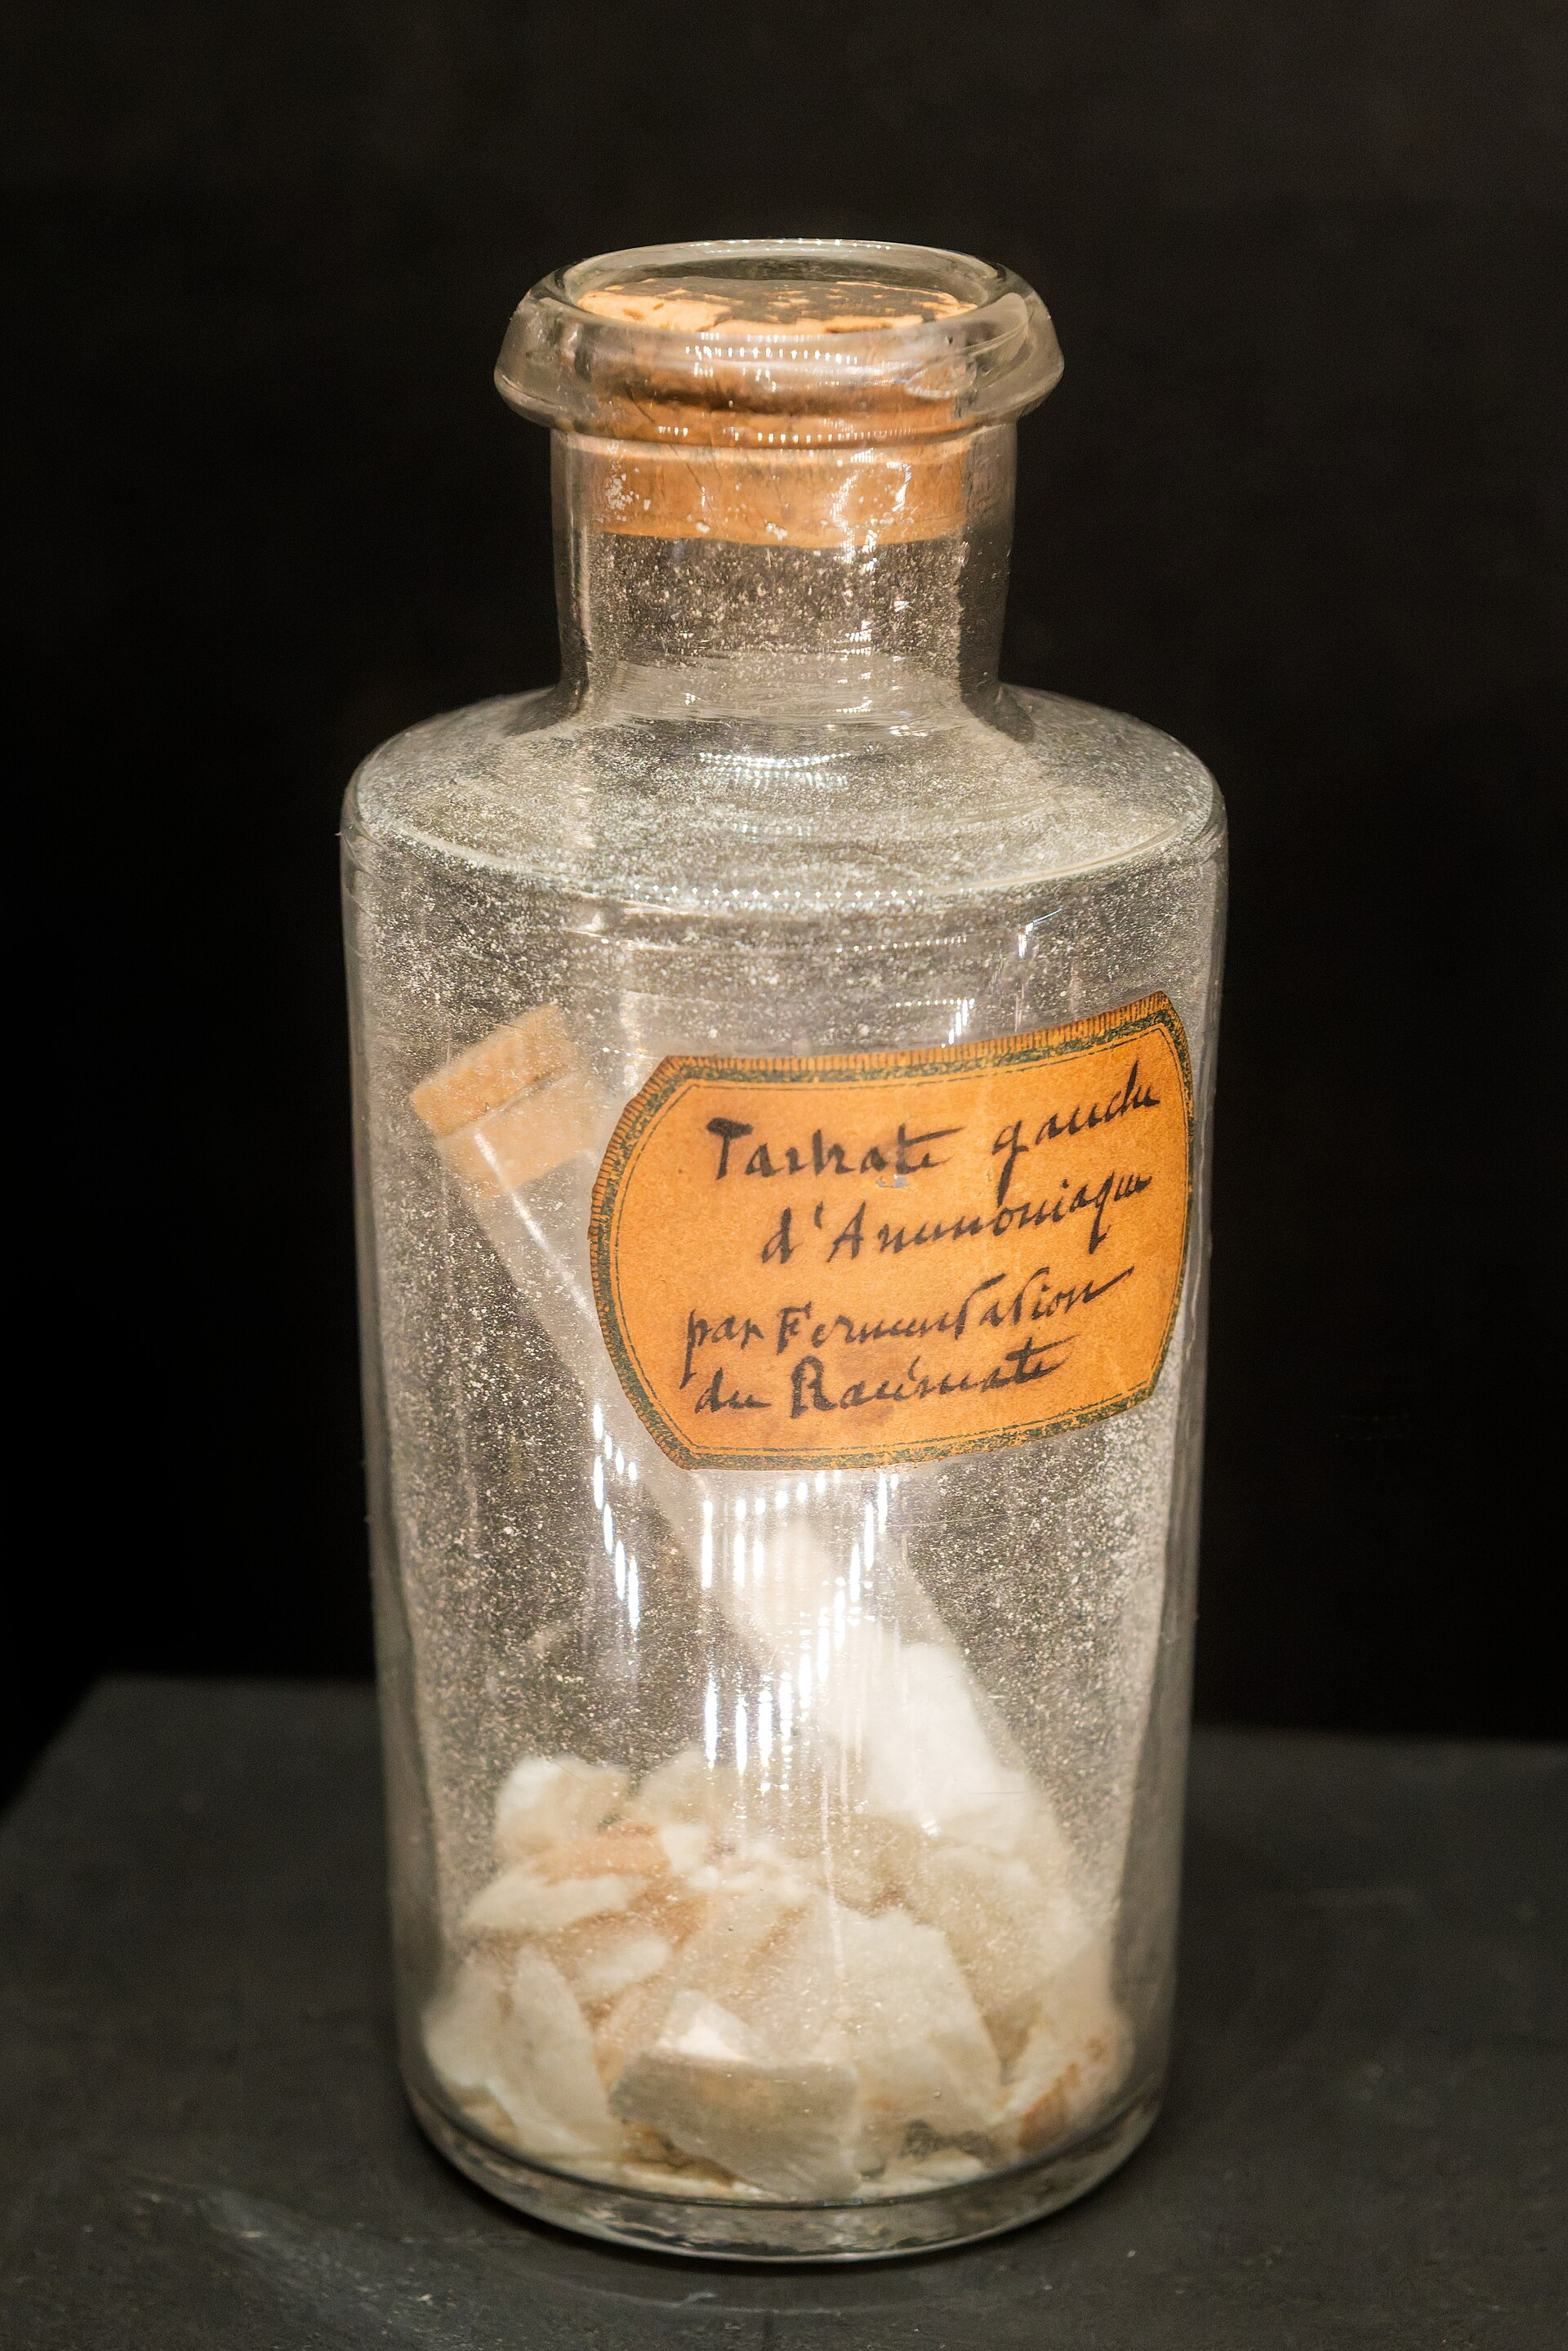
\includegraphics[height=5cm]{images/book1/tartrate-crystals.jpg}

{\small 巴斯德收藏的酒石酸铵晶体。
照片：Marie-Lan Taÿ Pamart，CC BY 4.0。}
\end{minipage}
\end{omfigure}

\section{Z 与 E 异构体}


\begin{definition}[Z 与 E 异构体]\label{def:g12:stereochemistry:z-e}
当 \ce{C=C} \omterm{def:g10:lewis-and-shape:multiple-bond}{双键}的每个碳\omterm{def:g7:atoms-and-molecules:atom}{原子}各连有两个不同的
\omterm{def:g7:atoms-and-molecules:atom}{原子}或基团时，存在两种\omterm{def:g12:stereochemistry:stereoisomer}{立体异构体}，
这是因为\omterm{def:g10:lewis-and-shape:multiple-bond}{双键}不能旋转。在每个碳\omterm{def:g7:atoms-and-molecules:atom}{原子}上，成键\omterm{def:g7:atoms-and-molecules:atom}{原子}的\omterm{def:g9:inside-the-atom:atomic-number}{原子序数}
较大的基团具有优先权。若两个优先基团位于\omterm{def:g10:lewis-and-shape:multiple-bond}{双键}的同侧，
则为 \emph{Z}\index{Z 异构体}；若位于异侧，
则为 \emph{E}\index{E 异构体}。
\end{definition}

\begin{method}[Z 还是 E？]\label{met:g12:stereochemistry:z-e}
\begin{enumerate}
  \item 检查\omterm{def:g10:lewis-and-shape:multiple-bond}{双键}的每个碳\omterm{def:g7:atoms-and-molecules:atom}{原子}是否各连有两个不同的
        基团；否则不存在 Z/E 异构现象。
  \item 在每个碳\omterm{def:g7:atoms-and-molecules:atom}{原子}上，优先选择首个\omterm{def:g7:atoms-and-molecules:atom}{原子}的
        \omterm{def:g9:inside-the-atom:atomic-number}{原子序数}较大的基团（并列时的完整规则见
        本科一年级分册）。
  \item 同侧为 Z，异侧为 E。
\end{enumerate}
\end{method}

\begin{omfigure}
\setchemfig{atom sep=2em}
\begin{tabular}{cc}
\chemfig{C(-[:150]H_3C)(-[:210]H)=C(-[:30]CH_3)(-[:-30]H)} &
\chemfig{C(-[:150]H_3C)(-[:210]H)=C(-[:30]H)(-[:-30]CH_3)} \\[4pt]
\small (Z)-2-丁烯：\ce{CH3} 基团位于同侧 &
\small (E)-2-丁烯：\ce{CH3} 基团位于异侧
\end{tabular}

{\small 2-丁烯的两种\omterm{def:g12:stereochemistry:stereoisomer}{立体异构体}。在每个碳\omterm{def:g7:atoms-and-molecules:atom}{原子}上，\ce{CH3}
（碳，$Z = 6$）优先于 \ce{H}（$Z = 1$）。二者互为
\omterm{def:g12:stereochemistry:diastereomer}{非对映异构体}，沸点各不相同。}
\end{omfigure}

\section{构象}

\begin{definition}[构象]\label{def:g12:stereochemistry:conformation}
\omterm{def:g7:atoms-and-molecules:molecule}{分子}中的\omterm{def:g7:atoms-and-molecules:atom}{原子}可绕单键旋转。每一种经旋转得到的
排列，都是该\omterm{def:g7:atoms-and-molecules:molecule}{分子}的\emph{构象}\index{构象}。
同一\omterm{def:g7:atoms-and-molecules:molecule}{分子}的不同构象不属于异构体，它们在室温下
不断地相互转化。
\end{definition}

\begin{omfigure}
\begin{tikzpicture}[font=\small]
  \pic (s) at (0,0) {omnewman={90}{30}};
  \foreach \k in {1,2,3} { \node at (s-f\k) {H}; \node at (s-b\k) {H}; }
  \node[anchor=north, align=center] at (0,-1.7) {交错式：两个碳原子的 H 原子 \\ 交替排列};
  \pic (e) at (5,0) {omnewman={90}{112}};
  \foreach \k in {1,2,3} { \node at (e-f\k) {H}; \node[black!60] at (e-b\k) {H}; }
  \node[anchor=north, align=center] at (5,-1.7) {重叠式：两组 H 原子相对 \\ （作图时略微分开）};
\end{tikzpicture}

{\small 乙烷（\ce{CH3-CH3}）的两种\omterm{def:g12:stereochemistry:conformation}{构象}，沿
\ce{C-C} 键观察：前端碳\omterm{def:g7:atoms-and-molecules:atom}{原子}为中心，后端碳\omterm{def:g7:atoms-and-molecules:atom}{原子}为圆周。
交错式\omterm{def:g12:stereochemistry:conformation}{构象}中\omterm{def:g7:atoms-and-molecules:atom}{原子}相距最远，是
最稳定的\omterm{def:g12:stereochemistry:conformation}{构象}。}
\end{omfigure}

\begin{remark}[为何重要]\label{rem:g12:stereochemistry:matters}
生物体由\omterm{def:g12:stereochemistry:chiral}{手性}\omterm{def:g7:atoms-and-molecules:molecule}{分子}（如蛋白质、糖类）构成，由它们组成的
受体和酶能够区分\omterm{def:g12:stereochemistry:enantiomer}{对映异构体}：两种
\omterm{def:g12:stereochemistry:enantiomer}{对映异构体}在气味、味道或药效上可能相差甚远。这就是为何
制造含\omterm{def:g12:stereochemistry:chiral}{手性碳原子}药物的化学家必须明确所制得的是哪种
\omterm{def:g12:stereochemistry:enantiomer}{对映异构体}，并对每一种分别进行检测。
\end{remark}

\section{练习}

\begin{exercise}[$\star$]\label{exo:g12:stereochemistry:1}
这些\omterm{def:g7:atoms-and-molecules:molecule}{分子}中哪些含有\omterm{def:g12:stereochemistry:chiral}{手性碳原子}？用星号标出。
2-丁醇 \ce{CH3-CH(OH)-CH2-CH3}；2-丙醇 \ce{CH3-CH(OH)-CH3}；
2-氯丁烷；乳酸 \ce{CH3-CH(OH)-COOH}。
\end{exercise}

\begin{exercise}[$\star$]\label{exo:g12:stereochemistry:2}
判断每一种异构体是 Z 型还是 E 型？
\begin{center}
\setchemfig{atom sep=1.8em}
\chemfig{C(-[:150]Cl)(-[:210]H)=C(-[:30]Cl)(-[:-30]H)} \qquad
\chemfig{C(-[:150]H_3C)(-[:210]H)=C(-[:30]H)(-[:-30]CH_2-CH_3)}
\end{center}
\end{exercise}

\begin{exercise}[$\star$]\label{exo:g12:stereochemistry:3}
下列物体中哪些具有\omterm{def:g12:stereochemistry:chiral}{手性}：手套、勺子、螺丝钉、正方体？
下列\omterm{def:g7:atoms-and-molecules:molecule}{分子}中，\ce{CH2Cl2} 和 \ce{CHFClBr} 哪一个具有\omterm{def:g12:stereochemistry:chiral}{手性}？
\end{exercise}

\begin{exercise}[$\star$]\label{exo:g12:stereochemistry:4}
什么是\omterm{def:g12:stereochemistry:enantiomer}{外消旋混合物}？以香芹酮为例，它闻起来是留兰香味、葛缕子味，
还是两者兼有？
\end{exercise}

\begin{exercise}[$\star$]\label{exo:g12:stereochemistry:5}
1-丁烯 \ce{CH2=CH-CH2-CH3} 能否存在 Z 型和 E 型异构体？为什么？
\end{exercise}

\begin{exercise}[$\star\star$]\label{exo:g12:stereochemistry:6}
用\omterm{def:g12:stereochemistry:cram}{楔形式}画出 2-丁醇的两种\omterm{def:g12:stereochemistry:enantiomer}{对映异构体}，
二者之间置一面镜子。
\end{exercise}

\begin{exercise}[$\star\star$]\label{exo:g12:stereochemistry:7}
下列物质各有多少种\omterm{def:g12:stereochemistry:stereoisomer}{立体异构体}：2-氯丁烷；
2,3-二氯丁烷 \ce{CH3-CHCl-CHCl-CH3}；2-戊烯
\ce{CH3-CH=CH-CH2-CH3}？
\end{exercise}

\begin{exercise}[$\star\star$]\label{exo:g12:stereochemistry:8}
判断下列各组是\omterm{def:g12:stereochemistry:enantiomer}{对映异构体}、\omterm{def:g12:stereochemistry:diastereomer}{非对映异构体}，还是同一\omterm{def:g7:atoms-and-molecules:molecule}{分子}：
L-酒石酸和 D-酒石酸；L-酒石酸和内消旋酒石酸；（Z）-与
（E）-2-丁烯；内消旋酒石酸与它自身的镜像。
\end{exercise}

\begin{exercise}[$\star\star$]\label{exo:g12:stereochemistry:9}
沿中心键观察丁烷 \ce{CH3-CH2-CH2-CH3}，画出
两个 \ce{CH3} 基团位于相对位置的交错式\omterm{def:g12:stereochemistry:conformation}{构象}，以及
一种两个基团彼此正对的重叠式\omterm{def:g12:stereochemistry:conformation}{构象}。哪一种更稳定？
为什么？
\end{exercise}

\begin{exercise}[$\star\star$]\label{exo:g12:stereochemistry:10}
内消旋酒石酸含有两个\omterm{def:g12:stereochemistry:chiral}{手性碳原子}，但不具有\omterm{def:g12:stereochemistry:chiral}{手性}。
试利用其对称面加以解释。
\end{exercise}

\begin{exercise}[$\star\star$]\label{exo:g12:stereochemistry:11}
画出 2-戊烯的 Z 型和 E 型异构体，并命名。
\end{exercise}

\begin{exercise}[$\star\star\star$]\label{exo:g12:stereochemistry:12}
2,3-二溴丁烷 \ce{CH3-CHBr-CHBr-CH3} 含有两个\omterm{def:g12:stereochemistry:chiral}{手性碳原子}。
用酒石酸所用的锯齿形式画出其\omterm{def:g12:stereochemistry:stereoisomer}{立体异构体}，
并证明其中一种为内消旋体。
\end{exercise}

\begin{exercise}[$\star\star\star$]\label{exo:g12:stereochemistry:13}
某药物\omterm{def:g7:atoms-and-molecules:molecule}{分子}含有一个\omterm{def:g12:stereochemistry:chiral}{手性碳原子}。其\omterm{def:g10:synthesis-yield:synthesis}{合成}得到\omterm{def:g12:stereochemistry:enantiomer}{外消旋混合物}，
但只有一种\omterm{def:g12:stereochemistry:enantiomer}{对映异构体}能与其所作用的\omterm{def:g12:stereochemistry:chiral}{手性}受体相匹配。
该外消旋药物中有多大比例具有活性？
给出化学家可以改进的两种方法。
\end{exercise}

\begin{exercise}[$\star\star\star$]\label{exo:g12:stereochemistry:14}
2,4-己二烯 \ce{CH3-CH=CH-CH=CH-CH3}，含有两个\omterm{def:g10:lewis-and-shape:multiple-bond}{双键}，每个\omterm{def:g10:lewis-and-shape:multiple-bond}{双键}
都可为 Z 型或 E 型。该\omterm{def:g7:atoms-and-molecules:molecule}{分子}有多少种\omterm{def:g12:stereochemistry:stereoisomer}{立体异构体}？（注意
\omterm{def:g7:atoms-and-molecules:molecule}{分子}的对称性。）
\end{exercise}

\begin{exercise}[$\star\star\star$]\label{exo:g12:stereochemistry:15}
某糖\omterm{def:g7:atoms-and-molecules:molecule}{分子}含有三个\omterm{def:g12:stereochemistry:chiral}{手性碳原子}，且不具有对称性。它最多可有多少
种\omterm{def:g12:stereochemistry:stereoisomer}{立体异构体}？这些\omterm{def:g12:stereochemistry:stereoisomer}{立体异构体}中有几对\omterm{def:g12:stereochemistry:enantiomer}{对映异构体}？
每一种\omterm{def:g12:stereochemistry:stereoisomer}{立体异构体}各有多少种\omterm{def:g12:stereochemistry:diastereomer}{非对映异构体}？
\end{exercise}

\section{问题：巴斯德的晶体}


\begin{problem}[{周末问题——酒石酸含有两个
手性碳原子：它实际有多少种立体异构体？}]
\label{pb:g12:stereochemistry:1}
% ledger: mp:tartaric-L, aw:C, aw:H, aw:O
酒石酸的各种形式，\ce{HOOC-CH(OH)-CH(OH)-COOH}，
在发现\omterm{def:g7:atoms-and-molecules:molecule}{分子}可具有\omterm{def:g12:stereochemistry:chiral}{手性}的过程中起了决定性作用。L-酒石酸约在 \qty{169}{\celsius} 熔化。

\medskip
\noindent\textbf{第一部分——\omterm{def:g7:atoms-and-molecules:molecule}{分子}。}
\begin{enumerate}
  \item 写出酒石酸的\omterm{def:g11:organic-skeletons:formulas}{分子式}及其\omterm{def:g10:the-mole:molar-mass}{摩尔质量}。
  \item 写出其\omterm{def:g11:functional-groups:functional-group}{官能团}的名称，并说明各有几个。
  \item 哪些碳\omterm{def:g7:atoms-and-molecules:atom}{原子}是\omterm{def:g12:stereochemistry:chiral}{手性}的？分别列出每个\omterm{def:g12:stereochemistry:chiral}{手性碳原子}所连的四个基团。
  \item 根据本章规则，它至多可有多少种
        \omterm{def:g12:stereochemistry:stereoisomer}{立体异构体}？
\end{enumerate}

\medskip
\noindent\textbf{第二部分——\omterm{def:g12:stereochemistry:stereoisomer}{立体异构体}。}
\begin{enumerate}[resume]
  \item 在 L-酒石酸的锯齿形画法中，\ce{OH} 基团
        画成实楔形还是虚楔形？
  \item 画出它的镜像。两者能否重合？
        为该镜像命名。
  \item 画出一个实楔与一个虚楔并存的形式。在脑海中绕
        中心键旋转该形式，并找出一个对称面。
  \item 该形式是否具有\omterm{def:g12:stereochemistry:chiral}{手性}？它叫什么名称？
  \item 解释为何酒石酸只有三种\omterm{def:g12:stereochemistry:stereoisomer}{立体异构体}。
  \item 判断 L 与 D、L 与内消旋体各自是
        \omterm{def:g12:stereochemistry:enantiomer}{对映异构体}还是\omterm{def:g12:stereochemistry:diastereomer}{非对映异构体}。
\end{enumerate}

\medskip
\noindent\textbf{第三部分——性质。}
\begin{enumerate}[resume]
  \item D-酒石酸在什么温度下熔化？为什么？
  \item 内消旋酒石酸是否必定在相同温度下熔化？为什么？
  \item 香芹酮表明两种\omterm{def:g12:stereochemistry:enantiomer}{对映异构体}的气味可以不同。为什么鼻子能够
        分辨它们，而温度计却不能？
  \item L 与 D 酒石酸的\omterm{def:g12:stereochemistry:enantiomer}{外消旋混合物}是否为
        \omterm{def:g6:pure-substances-and-mixtures:pure-substance}{纯净物}？整体上是否具有旋光性？
\end{enumerate}

\medskip
\noindent\textbf{第四部分——巴斯德。}
\begin{enumerate}[resume]
  \item 巴斯德所得的外消旋盐得到了两种互为镜像的晶体。
        每种晶体各含有什么？
  \item 若取 \qty{10.0}{g} 外消旋盐，他预期每种
        晶体的质量各为多少？
  \item 为什么内消旋体从不出现在这些晶体中？
  \item 分拣之后，他如何检验两堆晶体
        确为\omterm{def:g12:stereochemistry:enantiomer}{对映异构体}？
  \item 3-氯-2-丁醇 \ce{CH3-CHCl-CH(OH)-CH3} 同样含有两个
        \omterm{def:g12:stereochemistry:chiral}{手性碳原子}。它有多少种\omterm{def:g12:stereochemistry:stereoisomer}{立体异构体}？为什么它
        不会像酒石酸那样少掉一种？
  \item 给出最终答案：酒石酸共有多少种
        \omterm{def:g12:stereochemistry:stereoisomer}{立体异构体}？
\end{enumerate}
\end{problem}
